\documentclass[12pt,a4paper]{article}

\usepackage[pdftex]{graphicx}
%\usepackage{cite}
\usepackage{indentfirst}
\setlength{\parindent}{1em}
\usepackage{enumerate}
\usepackage{geometry}
\geometry{left=1in,right=1in,top=1in,bottom=1in}
%\usepackage{times}
%\usepackage{mathptmx}
\usepackage{listings}
\usepackage[framed,numbered,autolinebreaks,useliterate]{mcode}

\title{Lyapunov based Nonlinear Control - Assignment2}
\author{Sun Qinxuan}

\begin{document}
\maketitle

\section{Problem}

\indent Use Matlab/Simulink to simulate the following system
$$\dot{x}=-ax^3-b\sin{t}+u$$
$$e=x_d-d$$
$$x_d=\sin(t)$$
\begin{enumerate}[a)]
\item EMK Controller:
      $$u=[\dot{x_d}+ax^3+b\sin(t)]+ke$$
      adjust the control gain $k$ to make the tracking error go to zero, and then plot the figure of tracking error $e$ and control input $u$.
\item Adaptive Controller:
      $$u=[\dot{x_d}+\hat{a}x^3+\hat{b}\sin(t)]+ke$$
      $$\dot{\hat{a}}=\Gamma_1ex^3$$
      $$\dot{\hat{b}}=\Gamma_2e\sin(t)$$
      adjust the control gain $k$, parameter update gains $\Gamma_1$ and $\Gamma_2$ to make the tracking error go to zero and then plot the figure of tracking error $e$, parameters estimation $\hat{a}$, $\hat{b}$ and control input $u$.
\end{enumerate}

\section{Solution}

\indent Without loss of generality, we assume that $a=1.7$ and $b=-2.4$ for the system model.

\subsection{EMK controller}

\indent If the exact system model is available, the EMK controller can be applied to track the desired trajectory $x_d$. 

\indent Matlab ode45 function is used to simulate the control system as shown below.

\begin{lstlisting}
[t_ctl,y_ctl]=ode45(@emk_control,[0,last_time],x0,options);
\end{lstlisting}

where the emk\_control function as well as the sys\_model are defined accordingly.

\begin{lstlisting}
function dx=emk_control(t,x,a,b,k)
x_d=sin(t);
e=x_d-x;
dx_d=cos(t);
u=(dx_d+a*x^3+b*sin(t))+k*e;
dx=sys_model(t,x)+u;
\end{lstlisting}

\begin{lstlisting}
function dx=sys_model(t,x)
a=1.7;
b=-2.4;
dx=-a*x^3-b*sin(t);
\end{lstlisting}

\indent As shown in Table \ref{emk_table}, with the increasing $k$ value, the rate of convergence of the control system gets faster. Meanwhile, it requires fairly large control $u$ at the beginning when $k$ is set to a large value, as can be seen in Figure \ref{emk_fig}.

\subsection{Adaptive controller}

\indent For the systems which contain unknown parameters, the adaptive controller can be used rather than EMK controller to track the desired trajectory. Since $a$ and $b$ are unknown, so $\hat{a}$ and $\hat{b}$ are estimated online using the measured control error $e=x_d-x$ as the feedback. As a result, the estimated $\hat{a}$ and $\hat{b}$ are used in the feedforward part in the control variable rather than the exact system model.

\indent Similarly, the ode45 is used too with the derivative function substituted with adap\_control, which is defined below.

\begin{lstlisting}
function dx=adap_control(t,x,gamma1,gamma2,k)
% dx=[x_dot,a_dot,b_dot];
x_d=sin(t);
e=x_d-x(1);
dx_d=cos(t);
u=(dx_d+x(2)*x(1)^3+x(3)*sin(t))+k*e;
dx=[sys_model(t,x(1))+u;gamma1*e*x(1)^3;gamma2*e*sin(t)];
\end{lstlisting}

Note that the estimated parameters $\hat{a}$ and $\hat{b}$ are also the variables in the derivative equation, since they are adaptively adjusted while the system is running.

\indent Choose $k=5$ according to the results of the previous section. Firstly, we set the initial state of $\hat{a}=1$ and $\hat{b}=-2$ close to the true parameters in the system model. Let $\Gamma_1$ and $\Gamma_2$ be $1$ and $5$, and plot the figures for control performance in Figure \ref{adap1} and Figure \ref{adap2}, respectively. Then, change the the initial state as $\hat{a}=-1$ and $\hat{b}=3$ and show the control performance in Figure \ref{adap3}.

\indent From the results we can see that when adaptive controller is utilized, the control error $e$ tends to converge to zero exponentially fast but it shows the property of slight oscillation, which makes the control performance not as good as that of EMK controller. As for the estimated $\hat{a}$ and $\hat{b}$, they will stabilize at some certain values as time goes by. However, they are not ensured to converge to the true system parameters and might converge to different values when taking different initial states or update gain.

\begin{table}
% increase table row spacing, adjust to taste
%\renewcommand{\arraystretch}{1.3}
\caption{The convergence rate of control error $e$ w.r.t. the control gain $k$.}
\label{emk_table}
\centering
\begin{tabular}{lllllll}
\hline
k &0.5 &1 &5 &10 &20 &50\\
\hline
t (when $|e|$ reaches $10^{-3}$) &15.3	&7.6 &1.5 &0.76 &0.38 &0.15\\
\hline
\end{tabular}
\end{table}

\begin{figure}
\begin{minipage}{0.48\linewidth}\footnotesize
  \centerline{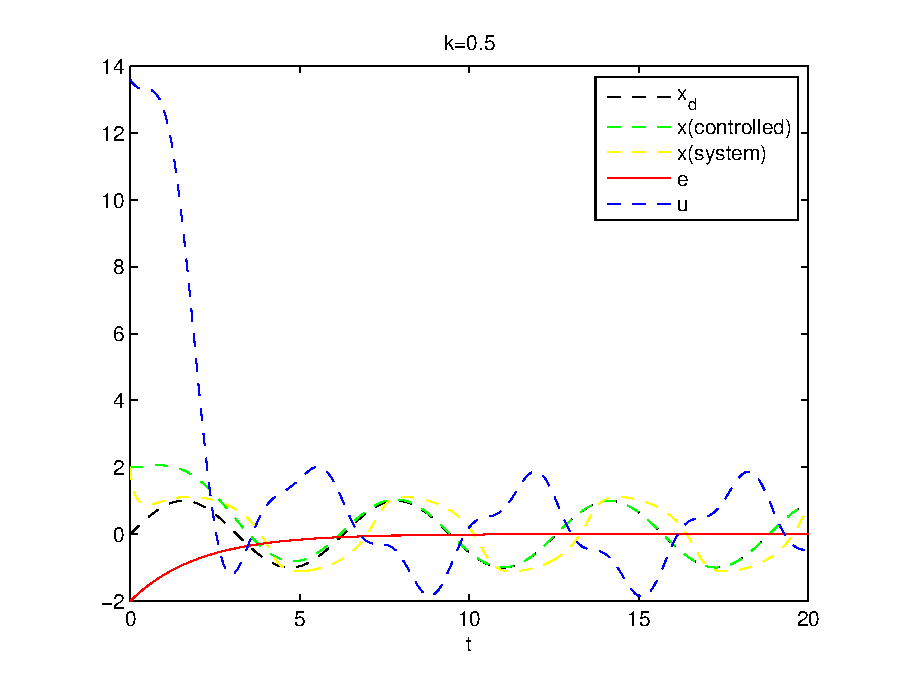
\includegraphics[width=7cm]{figs/emk0_5.eps}}
  \centerline{(a) $k$=0.5.}
\end{minipage}
\hfill
\begin{minipage}{0.48\linewidth}\footnotesize
  \centerline{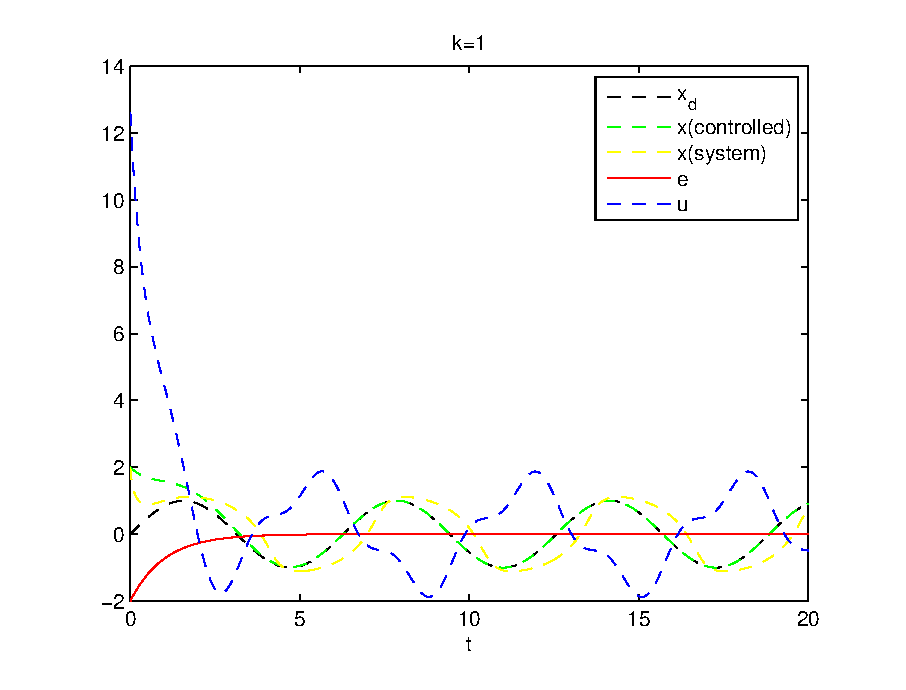
\includegraphics[width=7cm]{figs/emk1.eps}}
  \centerline{(b) $k$=1.}
\end{minipage}
\vfill
\begin{minipage}{0.48\linewidth}\footnotesize
  \centerline{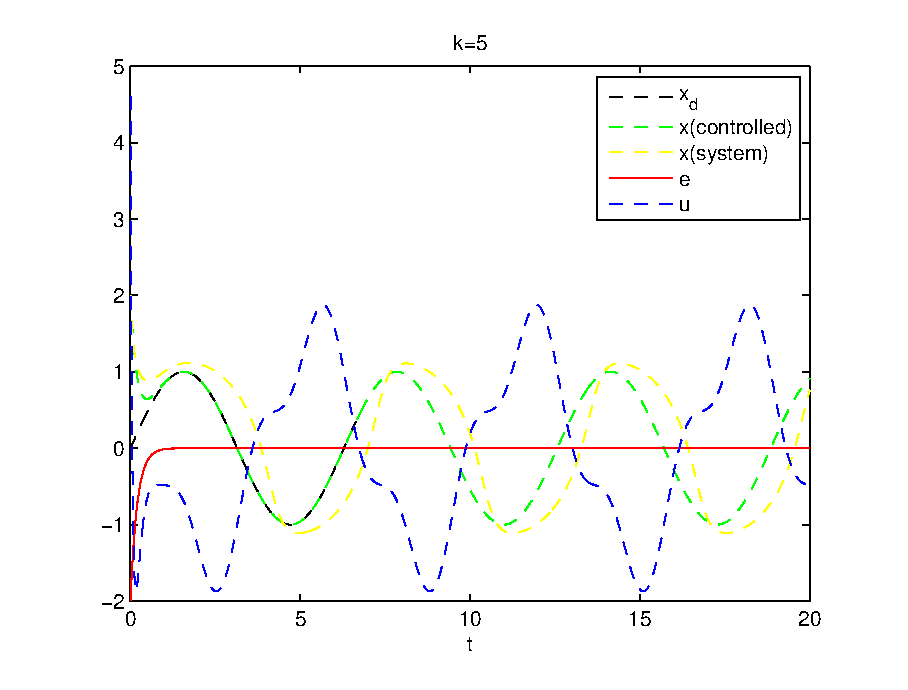
\includegraphics[width=7cm]{figs/emk5.eps}}
  \centerline{(c) $k$=5.}
\end{minipage}
\hfill
\begin{minipage}{0.48\linewidth}\footnotesize
  \centerline{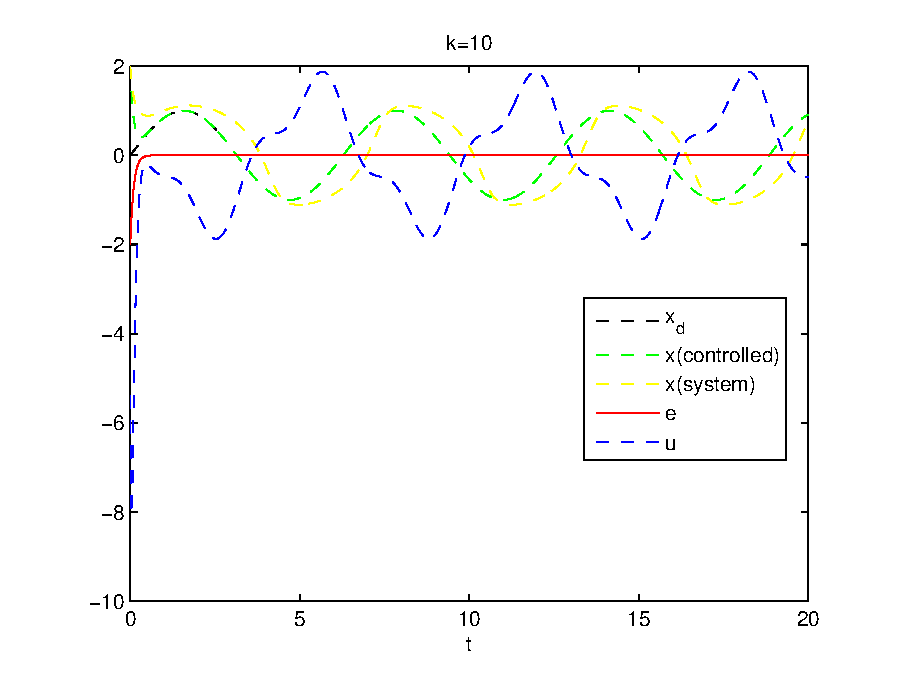
\includegraphics[width=7cm]{figs/emk10.eps}}
  \centerline{(d) $k$=10.}
\end{minipage}
\vfill
\begin{minipage}{0.48\linewidth}\footnotesize
  \centerline{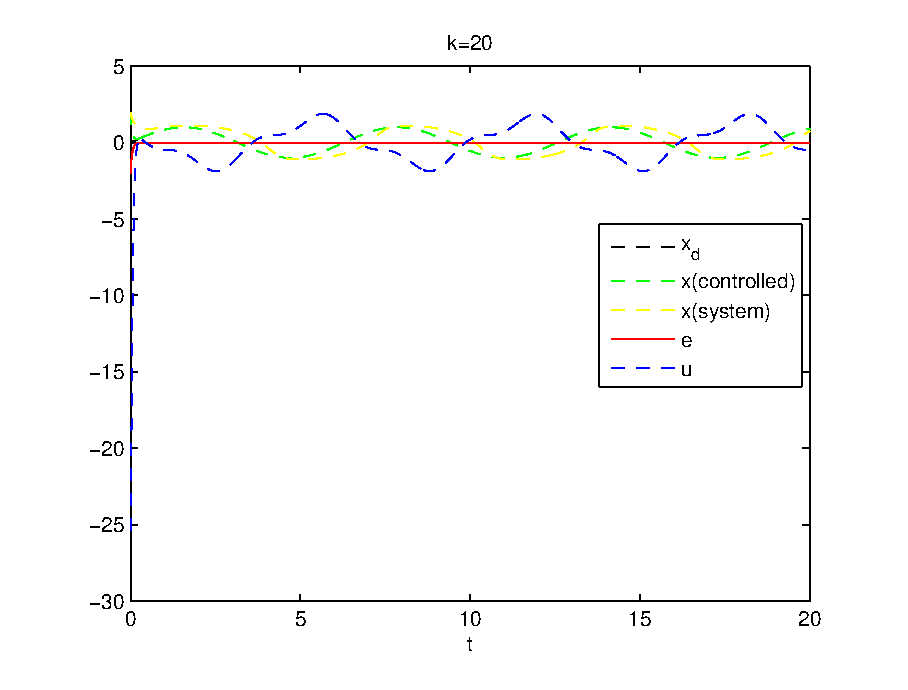
\includegraphics[width=7cm]{figs/emk20.eps}}
  \centerline{(e) $k$=20.}
\end{minipage}
\hfill
\begin{minipage}{0.48\linewidth}\footnotesize
  \centerline{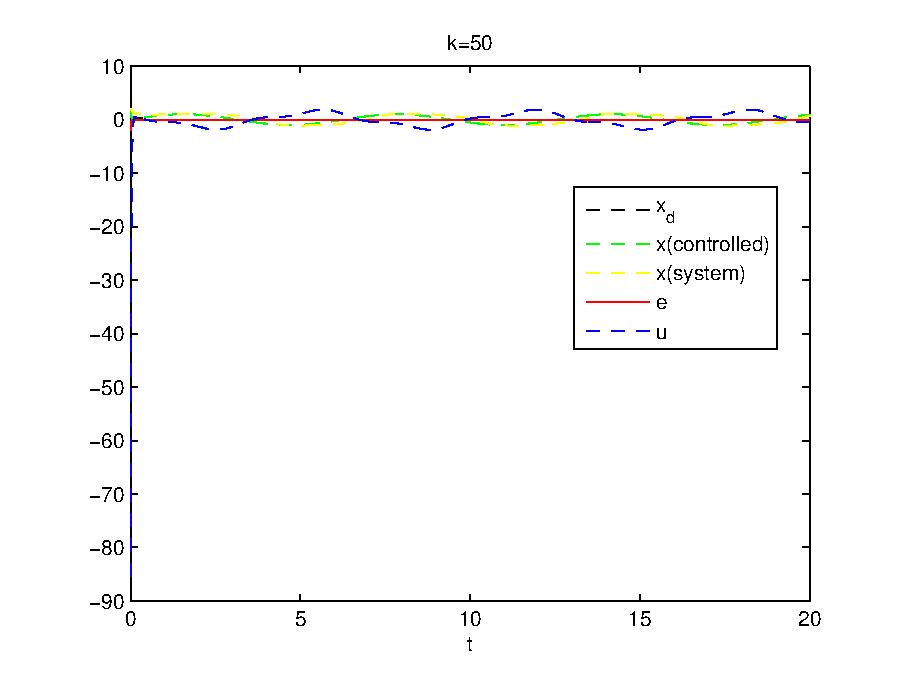
\includegraphics[width=7cm]{figs/emk50.eps}}
  \centerline{(f) $k$=50.}
\end{minipage}
\vfill
\caption{The performance of EMK controller for different $k$.}
\label{emk_fig}
\end{figure}

\begin{figure}
  \centering
  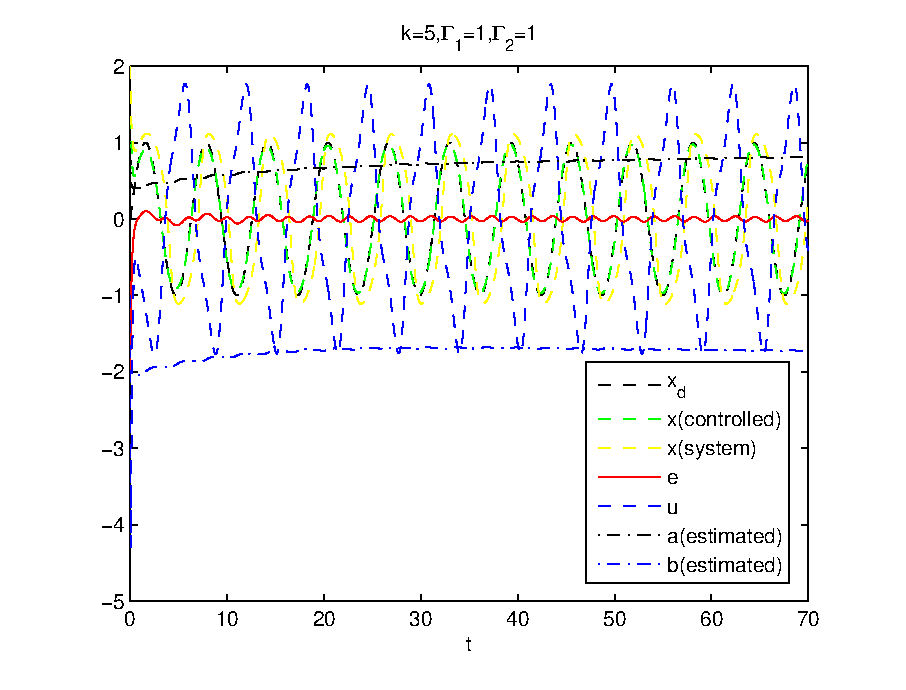
\includegraphics[width=0.8\textwidth]{figs/adap_1_init1.eps}% 1\linewidth
  \caption{Adaptive controller with $\Gamma_1=1$, $\Gamma_2=1$ and initial values $\hat{a}_0=1$ and $\hat{b}_0=-2$.}
  \label{adap1}
\end{figure}

\begin{figure}
  \centering
  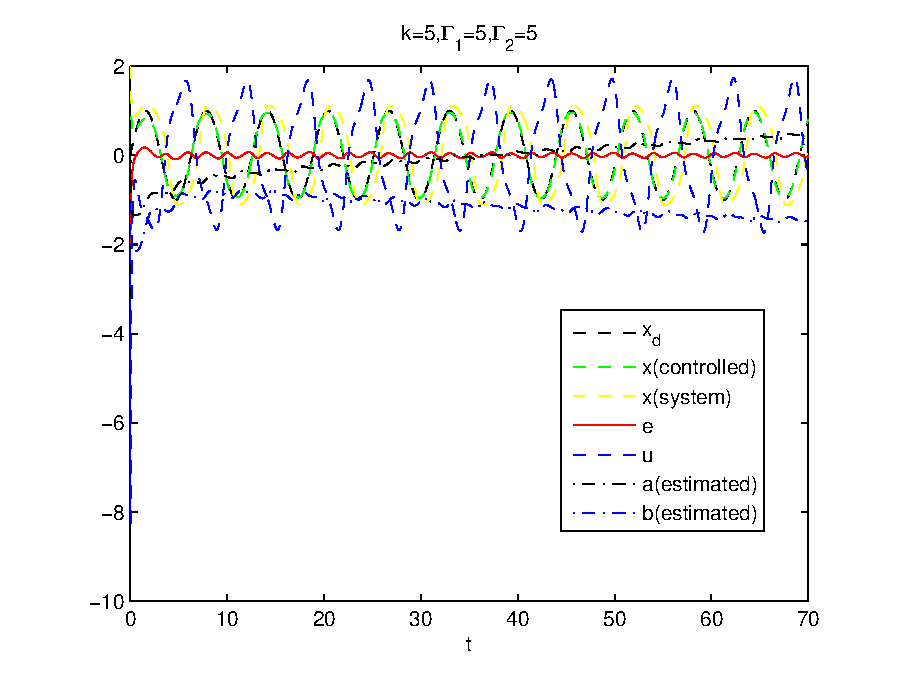
\includegraphics[width=0.8\textwidth]{figs/adap_5_init1.eps}% 1\linewidth
  \caption{Adaptive controller with $\Gamma_1=5$, $\Gamma_2=5$ and initial values $\hat{a}_0=1$ and $\hat{b}_0=-2$.}
  \label{adap2}
\end{figure}

\begin{figure}
  \centering
  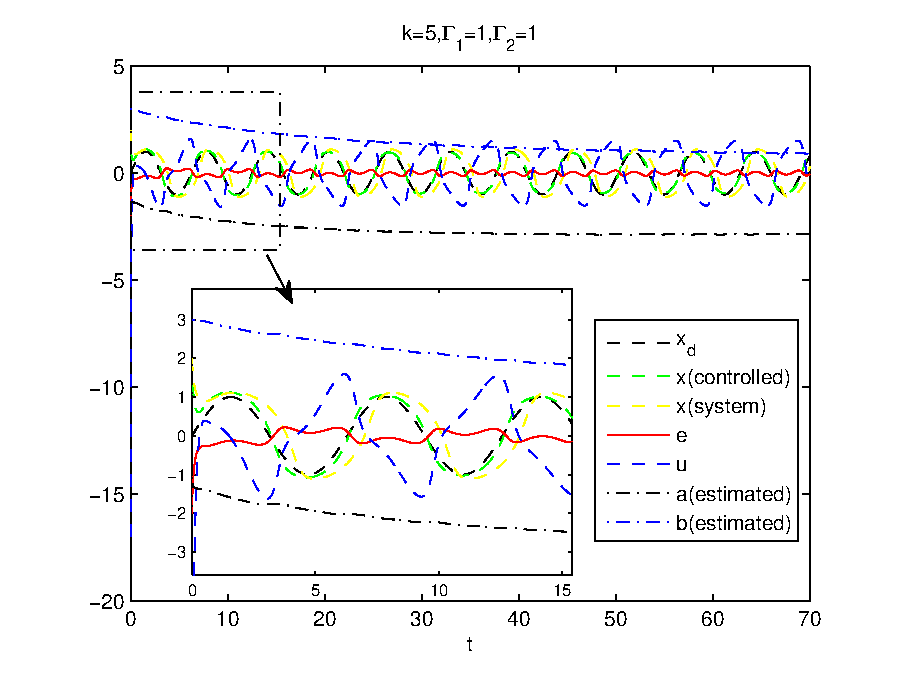
\includegraphics[width=0.8\textwidth]{figs/adap_1_init2.eps}% 1\linewidth
  \caption{Adaptive controller with $\Gamma_1=1$, $\Gamma_2=1$ and initial values $\hat{a}_0=-1$ and $\hat{b}_0=3$.}
  \label{adap3}
\end{figure}



\end{document} 